\subsection{Metadata labels}\label{sec:appendix_meta_data}

\subsubsection{Category}\label{subsec:appendix_category}

Here are the $58$ different categories, which make up all the category labels present within the dataset.
Categories with fewer than 139 documents ($0.1$ of the number of documents) are removed as part of preprocessing and replaced with a single misc category 'misc'.
This reduces the amount of categories to $34$, while only replacing 292 document's categories to 'misc'.
This preprocessing also makes the size of the remaining categories much more evenly distributed, as can be seen in \autoref{fig:category_hist}.

\begin{figure*}[ht]
	\centering
	\begin{subfigure}{0.45\textwidth}
		\centering
		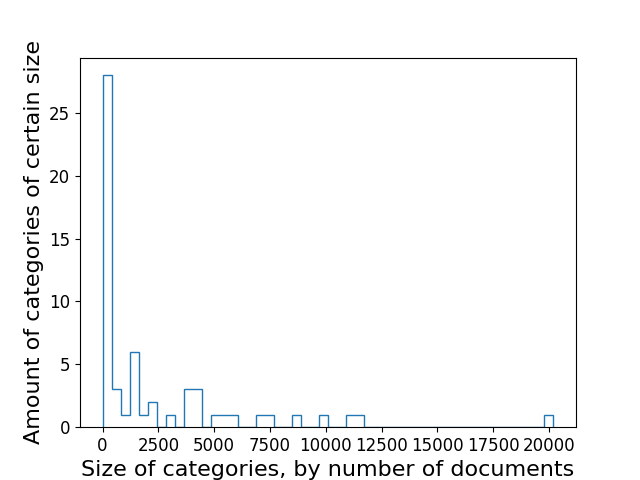
\includegraphics[width=\linewidth]{figures/category_hist2_before.png}
		\caption{Before preprocessing}
		\label{fig:category_hist_before}
	\end{subfigure}
	\begin{subfigure}{0.45\textwidth}
		\centering
		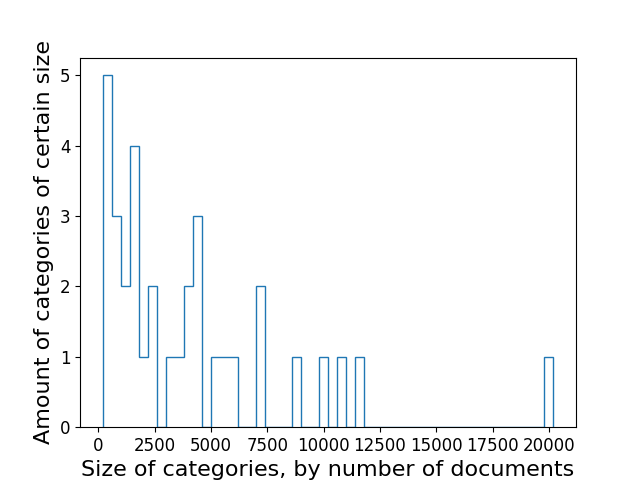
\includegraphics[width=\linewidth]{figures/category_hist2_140.png}
		\caption{After preprocessing}
		\label{fig:category_hist_after}
	\end{subfigure}
	\caption{Histogram over amount of categories different number of documents, before and after preprocessing. Categories in the x-axis are grouped into 50 buckets.}
	\label{fig:category_hist}
\end{figure*}


\begin{table*}[h]
	\centering
	\begin{tabular}{l|c|l|c|l|c|l|c}
		Category & Number & Category & Number & Category & Number & Category & Number \\
 		\toprule
		Udland-avis & 8855 & 26. Frederik & 484 & INFOMAKER PRINT* & 5 & Thisted sport & 698\\
		Kram & 244 & Feature & 188 & Thisted-net* & 3 & WEEKEND & 1493\\
		Navne & 3749 & Morsø-avis & 5959 & DF Licitation Diverse* & 4 & Erhverv-avis & 7356\\
		Brønderslev-net* & 1 & Aalborg-avis & 5544 & Oplandsavisen* & 6 & Biler* & 13\\
		Fælles & 20204 & Mariagerfjord-avis & 7241 & Morsø Sport & 2350 & Sport-net* & 3\\
		Bo Godt & 1447 & Erhvervsnavne* & 39 & Debat & 10075 & Frieord & 1341\\
		RB* & 3 & Hanbo-bladet* & 2 & Lokalavisen* & 1 & Indsigt & 984\\
		Samfund* & 9 & Morsø Debat & 1375 & Sport-avis & 10941 & Kultur & 3012 \\
		53. Frederik & 203 & DF Søfart* & 32 & Bagside & 1933 & Morsø-net* & 1 \\
		Frederikshavn-avis & 4325 & Nordjyske Biler & 1400 & Østvendsyssel Avis* & 4 & Aalborg:nu* & 73\\
		Perspektiv & 613 & Brønderslev-avis & 3857 & Rebild-avis & 4415 & Brugermappe* & 1\\
		Thisted-avis & 11473 & DF Motor Biler* & 3 & Nyhedsmotoren-net* & 3 & Morsø Ugeavis* & 27\\
		Jammerbugt-avis & 3791 & MitLiv & 1519 & Newspack* & 35 & DF Licitation Byggeri* & 14\\
		Mariagerfjord-net* & 1 & Hjørring-avis & 4235 & Friii & 2333 & Vesthimmerland-avis & 5131\\
		Plus Publicering* & 3 & Nordjyske Plus* & 6 & & & & \\
		\bottomrule
	\end{tabular}
	\caption{Amount of documents with each category within the Nordjyske dataset from 2017 to 2019. 
	Categories marked with * are removed as part of metadata preprocessing.}
	\label{tab:category_table}
\end{table*}


\subsubsection{Author}\label{subsec:appendix_author}
Unlike with Categories, the Author metadata field does not have a natural cut-off point, with a good amount of values in a specific lower range, followed by more evenly distributed numbers.
Instead, the vast majority of the values fall in a lower range, meaning that setting too high a cut-off point, will result in removing a large portion of the data.
We instead choose a lower cut-off point, keeping most of the authors, except the ones that contained so few documents, that finding common topics would be inefficient.
Authors who have written less that $14$ documents ($0.01\%$ of the number of documents) are removed as part of preprocessing.
This removes $43$ out of $227$ authors, combining them into a single 'misc' author.
A total of $204$ documents are assigned to the 'misc' author.
\todo[inline]{figure out whether to use boxplots or histograms, and ref them.}

\begin{figure*}[ht]
	\centering
	\begin{subfigure}{0.45\textwidth}
		\centering
		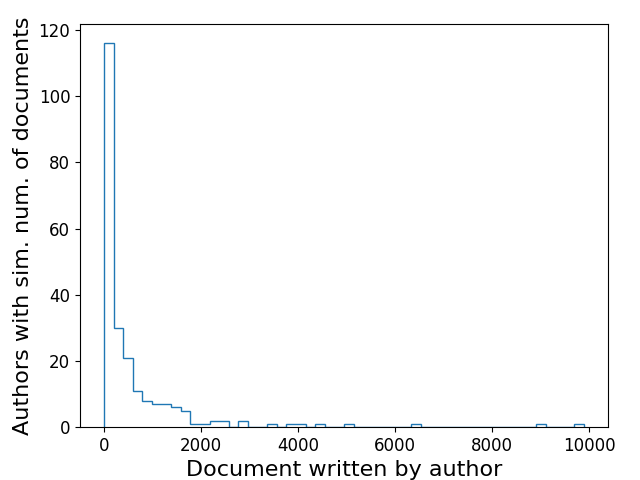
\includegraphics[width=\linewidth]{figures/author_hist2_before.png}
		\caption{Before preprocessing}
		\label{fig:author_hist_before}
	\end{subfigure}
	\begin{subfigure}{0.45\textwidth}
		\centering
		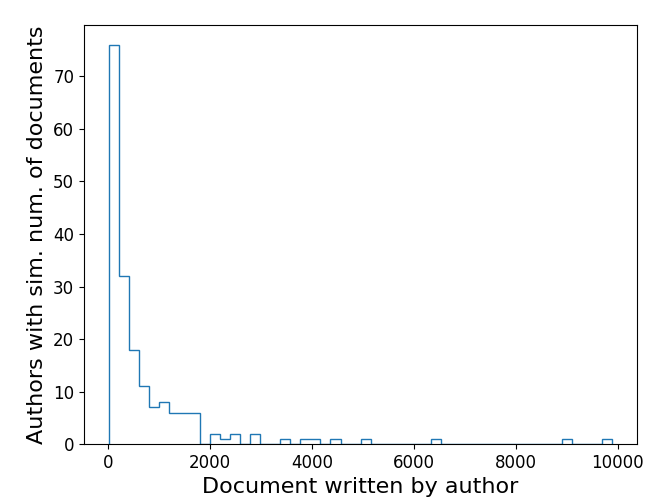
\includegraphics[width=\linewidth]{figures/author_hist2_14.png}
		\caption{After preprocessing}
		\label{fig:auhtor_hist_after}
	\end{subfigure}
	\caption{Histogram over amount authors who have written certain number of documents, before and after preprocessing. Authors in the x-axis are grouped into 50 buckets.}
	\label{fig:author_hist}
\end{figure*}

\begin{figure*}[ht]
	\centering
	\begin{subfigure}{0.45\textwidth}
		\centering
		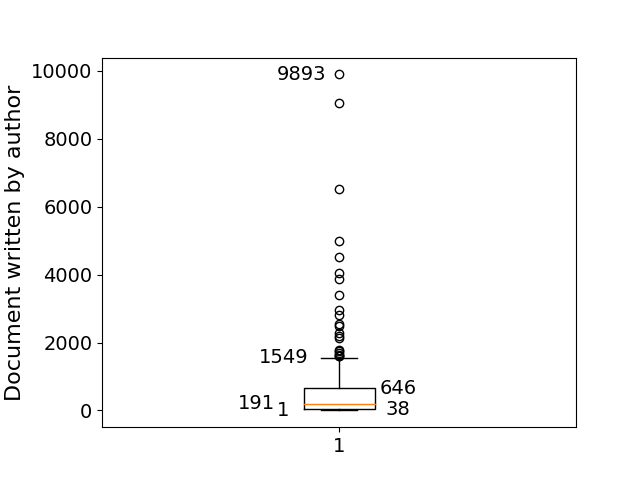
\includegraphics[width=\linewidth]{figures/author_box_before.png}
		\caption{Before preprocessing}
		\label{fig:author_box_before}
	\end{subfigure}
	\begin{subfigure}{0.45\textwidth}
		\centering
		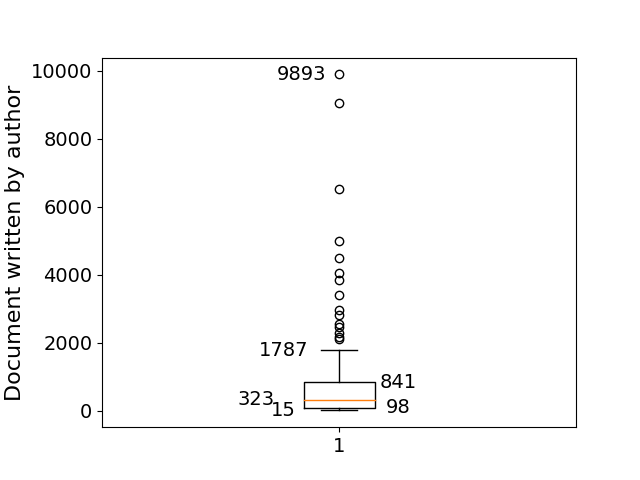
\includegraphics[width=\linewidth]{figures/author_box_14.png}
		\caption{After preprocessing}
		\label{fig:auhtor_box_after}
	\end{subfigure}
	\caption{Boxplot over the amount of documents written by authors.}
	\label{fig:author_box}
\end{figure*}

\subsubsection{Taxonomy}\label{subsec:appendix_taxonomy}
Taxonomy is fundamentally different from the other metadata fields, in this paper.
It is not fully observed with only roughly $25\%$ of documents having a taxonomy field.
It is hierarchical, with each taxonomy containing a sequence of sub-taxonomies, such as: 'STEDER/Danmark/Nordjylland/Aalborg'.
It is also possible for each document to have multiple taxonomy sequences.
We remove any sub-taxonomy that is used in less than $4$ taxonomy sequences.
Out of $1135$ sub-taxonomies, $522$ are removed during this preprocessing.
\todo[inline]{describe layer sizes of taxonomy tree}

\begin{table}
	\begin{tabular}{l | c | c | c | c | c}
		Metadata & Min & Max & Mean & Median & Std. \\
		\hline
		Author & 1 & 9893 & 612.6 & 191 & 1219.7 \\
		Author (preprocessed) & 15 & 9893 & 751.7 & 323 & 1311.9 \\
		Category & 1 & 20204 & 2397.6 & 548 & 3812.1 \\
		Category (preprocessed) & 188 & 20204 & 4090.0 & 2681 & 4227.3 \\
		Taxonomy & 1 & 29535 & 123.0 & 6 & 1385.9 \\
		Taxonomy (preprocessed) & 5 & 29535 & 227.6 & 17 & 1879.2 \\
	\end{tabular}
	\caption{Statistics over documents associated with metadata values, before and after preprocessing}
	\label{tab:meta_prepro_stats}
\end{table}
